\documentclass[]{article}
\usepackage{hyperref}
\usepackage{graphicx}
\usepackage{float}
\usepackage{amsmath}
\usepackage{amssymb}
\usepackage[ngerman]{babel}
\usepackage[T1]{fontenc}
\usepackage{lmodern}
\usepackage[utf8]{inputenc} % unter Windows latin1 statt utf8

%opening
\title{Farmrobo}

\author{Jonas Kallweidt und Christian Küllmer}
\date{\today{}, Kassel}

\begin{document}
\maketitle
\begin{figure}[H]
	\centering
	
\includegraphics[width=0.8\textwidth]{DeckblattFarmrobo.jpg}
	\caption{Automatik in der Landwirtschaft}
	\label{img:grafik-dummy}
\end{figure}
\newpage
\tableofcontents


\begin{abstract}
	

\end{abstract}

\section{Vorwort}

	\begin{figure}[H]
	\centering
	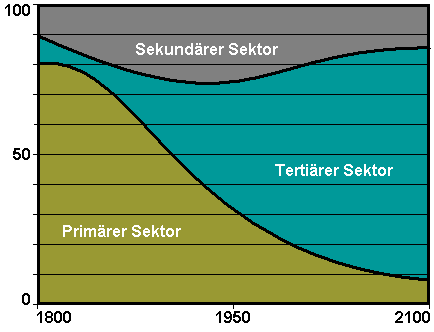
\includegraphics[width=0.8\textwidth]{Fourastie.png}
	\caption{Anzeige der Verteilung von Arbeitskräften zur Zeit \newline
		Quelle: Jean Fourastié: Le Grand Espoir du XXe siècle. Progrès technique, progrès économique, progrès social. Presses Universitaires de France, Paris 1949 = Die große Hoffnung des 20. Jahrhunderts. Köln 1954.}
	\
	\label{img:grafik-dummy}
	
\end{figure} 



Die Konzeption zu automatisiertem Gemüseanbau hat ihren Ursprung in der Tatsache, dass seit der Industrialisierung der Arbeitskräftebedarf der Landwirtschaft zwar schrumpft aber bis heute auf einem stabilen Niveau angekommen ist. Während viele Bereiche des Sekundärsektors durch Maschinen, bei sinkendem Bedarf an Arbeitskraft, bereits größere Produktivität entfalten so ist der Gemüseanbau noch mit großem manuellen Aufwand verbunden. 

Diese Personalkosten haben ein enormes Einsparpotential, während fachlich qualifizierte Spezialisten ihr Fachwissen zu einer breiten Anwendung bringen können.
In dieser Projektarbeit soll gezeigt werden, dass es zu diesem Zeitpunkt noch ein großes Potential bei (ggf. regionalem und von Arbeitskräften unabhängigem) Gemüseanbau gibt, welches durch automatisierten Gemüseanbau nutzbar gemacht werden kann. Es soll untersucht werden, welche Bestandteile für eine Pflanze die wichtigsten Parameter sind um sich entwickeln zu können. Diese Parameter sollen messbar gemacht und die Daten dieser Messung digital gespeichert werden. Diese Speicherbarkeit soll die Einstellung der Parameter möglich machen, wobei sich ebenfalls mit der Wirkbarkeit der Parameter auf die Pflanze beschäftigt werden soll. All dies soll aus dem Hinblick betrachtet werden ein Feld oder einen Zucht Rahmen für Pflanzen vollständig zu automatisieren.

In der aktuellen Forschungsdebatte gibt es bisher keine Möglichkeit automatisiert Gemüse anzubauen. Zwar gibt es Konzepte, wie den Farmbot oder den Farmduino, diese sehen Gemüseanbau allerdings nicht aus der Sicht der vollständigen industriellen Umsetzbarkeit, sondern eher im Hobbybereich einzelne Tätigkeiten Zeit/Software gesteuert an eine Maschine zu übergeben. Diese Konzepte haben allerdings ein großes Potential zu Optimierung. Die Entscheidung eine eigene Maschine zu entwickeln wurde davon bestärkt, dass hier die Möglichkeiten von maschinellem Lernen, Bilderkennung und der vollständigen Automation des Gemüseanbaus Raum gegeben werden kann. Es geht in diesem Projekt darum ein Trägersystem für verschiedenste Implementierungen zu entwickeln. Es soll die Anbindungsmöglichkeit zu neuronalen Netzen der ersten und zweiten Ebene entstehen. Daraus resultieren die Möglichkeiten, dass der Gemüseanbau durch sammlung von Daten stark optimiert und der Output eines Feldes unter umständen stark gesteigert werden kann. Der Ansatz ist von daher neu, weil hier zum ersten mal Formen der E-Technik und der Informatik hier als technisches Mittel Anwendung finden und im Zentrum der Automatisierung stehen. Die Methoden der Agrarkultur-Haltung werden hierbei nur zum Mittel der Pflanzenzucht eingesetzt. 

Motivation:
Warum ist automation in der Landwirtschaft so wichtig?

	\begin{figure}[H]
	\centering
	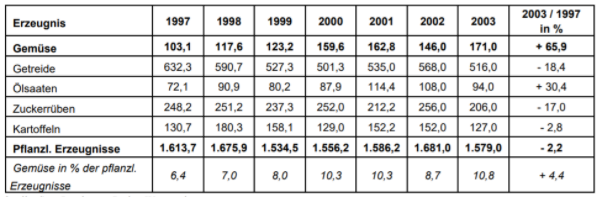
\includegraphics[width=0.8\textwidth]{Tabelle_Daten_Produktion.PNG}
	\caption{Anzeige der Verteilung von Arbeitskräften zur Zeit \newline
		Quelle Statl. Landesamt Baden-Wüttemberg Zitierte Quelle Online im Internet:
		\url{ https://www.lfl.bayern.de/mam/cms07/publikationen/daten/informationen/p_19984.pdf}}
	\label{img:grafik-dummy}
	
\end{figure} 

Es kann festgestellt werden, dass die erlöse der regionalen Landwirtschaft immer weiter steigen. eine weitgehende Automatisierung kann hier zu noch höheren Gewinnspannen führen.

\subsection{Motivation für das Farmrobo Projekt}


\section{Systemarchitektur}

\subsection{Überlegungen}
Die Datenverarbeitung bei der Farmrobomaschine soll dezentral erfolgen.







\end{document}
